\documentclass[12pt,a4paper]{article}
\usepackage{lmodern}

\usepackage{enumitem}
\usepackage{placeins}
\usepackage{amssymb,amsmath}
\usepackage{ifxetex,ifluatex}
\usepackage{fixltx2e} % provides \textsubscript
\ifnum 0\ifxetex 1\fi\ifluatex 1\fi=0 % if pdftex
  \usepackage[T1]{fontenc}
  \usepackage[utf8]{inputenc}
\else % if luatex or xelatex
  \ifxetex
    \usepackage{mathspec}
    \usepackage{xltxtra,xunicode}
  \else
    \usepackage{fontspec}
  \fi
  \defaultfontfeatures{Mapping=tex-text,Scale=MatchLowercase}
  \newcommand{\euro}{€}
\fi
% use upquote if available, for straight quotes in verbatim environments
\IfFileExists{upquote.sty}{\usepackage{upquote}}{}
% use microtype if available
\IfFileExists{microtype.sty}{%
\usepackage{microtype}
\UseMicrotypeSet[protrusion]{basicmath} % disable protrusion for tt fonts
}{}
\usepackage[lmargin = 2cm, rmargin = 2cm, tmargin = 2cm, bmargin = 2.5cm]{geometry}


% Figure Placement:
\usepackage{float}
\let\origfigure\figure
\let\endorigfigure\endfigure
\renewenvironment{figure}[1][2] {
    \expandafter\origfigure\expandafter[H]
} {
    \endorigfigure
}

%%%% Jens %%%%
\usepackage{titlesec}
\DeclareMathOperator*{\argmax}{arg\,max}
\DeclareMathOperator*{\argmin}{arg\,min}
\renewcommand{\vec}{\operatorname{vec}}
\newcommand{\tr}{\operatorname{tr}}
\newcommand{\Var}{\operatorname{Var}} % Variance
\newcommand{\MSE}{\operatorname{MSE}} % Variance
\newcommand{\VAR}{\operatorname{VAR}} % Vector autoregression
\newcommand{\Lag}{\operatorname{L}} % Lag operator
\newcommand{\Cov}{\operatorname{Cov}}
\newcommand{\diag}{\operatorname{diag}}
\newcommand{\adj}{\operatorname{adj}}
\newcommand{\loglik}{\operatorname{ll}}

\usepackage{centernot}

\allowdisplaybreaks

\titleformat{\section}
{\normalfont\large\bfseries}{\thesection}{1em}{}

\newcommand{\tmpsection}[1]{}
\let\tmpsection=\section
\renewcommand{\section}[1]{\tmpsection{\underline{#1}} }





%% citation setup
\usepackage{csquotes}

\usepackage[backend=biber, maxbibnames = 99, style = apa]{biblatex}
\setlength\bibitemsep{1.5\itemsep}
\addbibresource{R_packages.bib}
\usepackage{color}
\usepackage{fancyvrb}
\newcommand{\VerbBar}{|}
\newcommand{\VERB}{\Verb[commandchars=\\\{\}]}
\DefineVerbatimEnvironment{Highlighting}{Verbatim}{commandchars=\\\{\}}
% Add ',fontsize=\small' for more characters per line
\usepackage{framed}
\definecolor{shadecolor}{RGB}{248,248,248}
\newenvironment{Shaded}{\begin{snugshade}}{\end{snugshade}}
\newcommand{\AlertTok}[1]{\textcolor[rgb]{0.94,0.16,0.16}{#1}}
\newcommand{\AnnotationTok}[1]{\textcolor[rgb]{0.56,0.35,0.01}{\textbf{\textit{#1}}}}
\newcommand{\AttributeTok}[1]{\textcolor[rgb]{0.77,0.63,0.00}{#1}}
\newcommand{\BaseNTok}[1]{\textcolor[rgb]{0.00,0.00,0.81}{#1}}
\newcommand{\BuiltInTok}[1]{#1}
\newcommand{\CharTok}[1]{\textcolor[rgb]{0.31,0.60,0.02}{#1}}
\newcommand{\CommentTok}[1]{\textcolor[rgb]{0.56,0.35,0.01}{\textit{#1}}}
\newcommand{\CommentVarTok}[1]{\textcolor[rgb]{0.56,0.35,0.01}{\textbf{\textit{#1}}}}
\newcommand{\ConstantTok}[1]{\textcolor[rgb]{0.00,0.00,0.00}{#1}}
\newcommand{\ControlFlowTok}[1]{\textcolor[rgb]{0.13,0.29,0.53}{\textbf{#1}}}
\newcommand{\DataTypeTok}[1]{\textcolor[rgb]{0.13,0.29,0.53}{#1}}
\newcommand{\DecValTok}[1]{\textcolor[rgb]{0.00,0.00,0.81}{#1}}
\newcommand{\DocumentationTok}[1]{\textcolor[rgb]{0.56,0.35,0.01}{\textbf{\textit{#1}}}}
\newcommand{\ErrorTok}[1]{\textcolor[rgb]{0.64,0.00,0.00}{\textbf{#1}}}
\newcommand{\ExtensionTok}[1]{#1}
\newcommand{\FloatTok}[1]{\textcolor[rgb]{0.00,0.00,0.81}{#1}}
\newcommand{\FunctionTok}[1]{\textcolor[rgb]{0.00,0.00,0.00}{#1}}
\newcommand{\ImportTok}[1]{#1}
\newcommand{\InformationTok}[1]{\textcolor[rgb]{0.56,0.35,0.01}{\textbf{\textit{#1}}}}
\newcommand{\KeywordTok}[1]{\textcolor[rgb]{0.13,0.29,0.53}{\textbf{#1}}}
\newcommand{\NormalTok}[1]{#1}
\newcommand{\OperatorTok}[1]{\textcolor[rgb]{0.81,0.36,0.00}{\textbf{#1}}}
\newcommand{\OtherTok}[1]{\textcolor[rgb]{0.56,0.35,0.01}{#1}}
\newcommand{\PreprocessorTok}[1]{\textcolor[rgb]{0.56,0.35,0.01}{\textit{#1}}}
\newcommand{\RegionMarkerTok}[1]{#1}
\newcommand{\SpecialCharTok}[1]{\textcolor[rgb]{0.00,0.00,0.00}{#1}}
\newcommand{\SpecialStringTok}[1]{\textcolor[rgb]{0.31,0.60,0.02}{#1}}
\newcommand{\StringTok}[1]{\textcolor[rgb]{0.31,0.60,0.02}{#1}}
\newcommand{\VariableTok}[1]{\textcolor[rgb]{0.00,0.00,0.00}{#1}}
\newcommand{\VerbatimStringTok}[1]{\textcolor[rgb]{0.31,0.60,0.02}{#1}}
\newcommand{\WarningTok}[1]{\textcolor[rgb]{0.56,0.35,0.01}{\textbf{\textit{#1}}}}
\usepackage{graphicx}
\makeatletter
\def\maxwidth{\ifdim\Gin@nat@width>\linewidth\linewidth\else\Gin@nat@width\fi}
\def\maxheight{\ifdim\Gin@nat@height>\textheight\textheight\else\Gin@nat@height\fi}
\makeatother
% Scale images if necessary, so that they will not overflow the page
% margins by default, and it is still possible to overwrite the defaults
% using explicit options in \includegraphics[width, height, ...]{}
\setkeys{Gin}{width=\maxwidth,height=\maxheight,keepaspectratio}
\ifxetex
  \usepackage[setpagesize=false, % page size defined by xetex
              unicode=false, % unicode breaks when used with xetex
              xetex]{hyperref}
\else
  \usepackage[unicode=true, linktocpage = TRUE]{hyperref}
\fi
\hypersetup{breaklinks=true,
            bookmarks=true,
            pdfauthor={Dr.~Yannick Hoga},
            pdftitle={Multivariate Time Series Analysis},
            colorlinks=true,
            citecolor=black,
            urlcolor=black,
            linkcolor=black,
            pdfborder={0 0 0}}
\urlstyle{same}  % don't use monospace font for urls
\setlength{\parindent}{0pt}
\setlength{\parskip}{6pt plus 2pt minus 1pt}
\setlength{\emergencystretch}{3em}  % prevent overfull lines
\setcounter{secnumdepth}{5}

%%% Use protect on footnotes to avoid problems with footnotes in titles
\let\rmarkdownfootnote\footnote%
\def\footnote{\protect\rmarkdownfootnote}

%%% Change title format to be more compact
\usepackage{titling}

% Create subtitle command for use in maketitle
\newcommand{\subtitle}[1]{
  \posttitle{
    \begin{center}\large#1\end{center}
    }
}

\setlength{\droptitle}{-2em}
  \title{Multivariate Time Series Analysis}
  \pretitle{\vspace{\droptitle}\centering\huge}
  \posttitle{\par}
\subtitle{Solution Exercise Sheet 6}
  \author{Dr.~Yannick Hoga}
  \preauthor{\centering\large\emph}
  \postauthor{\par}
  \date{}
  \predate{}\postdate{}


%% linespread settings

\usepackage{setspace}

\onehalfspacing


% Language Setup

\usepackage{ifthen}
\usepackage{iflang}
\usepackage[super]{nth}
\usepackage[ngerman, english]{babel}

%Acronyms
\usepackage[printonlyused, withpage, nohyperlinks]{acronym}
\usepackage{changepage}

% Multicols for the Title page
\usepackage{multicol}


% foot


\begin{document}

\selectlanguage{english}

%%%%%%%%%%%%%% Jens %%%%%
\numberwithin{equation}{section}




\restoregeometry


%%% Header 

\begin{minipage}{0.6\textwidth}
University of Duisburg-Essen\\
Faculty of Business Administration and Economics\\
Chair of Econometrics\\
\end{minipage}

%\begin{minipage}{0.4\textwidth}
	\begin{flushright}
	\vspace{-3cm}
	\includegraphics*[width=5cm]{../Includes/duelogo_en.png}\\
	\vspace{.125cm}
	\end{flushright}
%\end{minipage}
%\vspace{.125cm}
\hspace{-0.005cm}Winter Term 2019/2020

\vspace{0.05cm}

\begin{center}
	\vspace{.25cm}
	Dr.~Yannick Hoga \hspace{.5cm} Thilo Reinschlüssel \\
	\vspace{.25cm}
	\textbf{\Large{Multivariate Time Series Analysis}}\\
	\vspace{.25cm}
	\textbf{\large{Solution Exercise Sheet 6}}\\
	\vspace{.125cm}
\end{center}




% body from markdown

\hypertarget{exercise-1-model-selection---review}{%
\section{Exercise 1: Model Selection -
Review}\label{exercise-1-model-selection---review}}

\begin{itemize}
  \item[a)] Is the MSE scale-invariant? 
\end{itemize}

\emph{Solution:}

No, the MSE is scale-dependent. Take the following \(\VAR(1)\) as an
example (\(\mu_z = 0 \ \text{w.l.o.g}\)):

\begin{align*}
z_t =  \phi_1 z_{t-1} + a_t\\
\end{align*}

Define \(k_t := b z_t\) where \(b\) is a scalar.

\begin{align*}
  \Rightarrow k_t & = b z_t = \phi_1 b z_{t-1} + e_t \\
  \Leftrightarrow e_T & = k_t - \phi_1 k_t = b \cdot \left(z_t - \phi z_{t-1} \right) = b \cdot a_t\\
  \\
  \MSE(\hat{k}_{t, t+1} ) & = \mathbb{E} \left[ e_{t+1}^{2}\right] = \mathbb{E} \left[ (b a_{t+1})^{2}\right] \\
   & = b^2 \cdot \mathbb{E} \left( a_{t+1}^{2}\right)\\
   & = b^2 \cdot  \MSE(\hat{z}_{t, t+1} )\\
\end{align*}

where \(\hat{k}_{t, t-1}, \hat{z}_{t, t-1}\) are the \(\VAR (1)\)
predictions.

\begin{itemize}
  \item[b)] What is the fundamental trade-off which information criteria are supposed to balance? 
\end{itemize}

\emph{Solution:}

\begin{align*}
  IC (l) & = \underbrace{\log \left( A \right)}_{\substack{\text{Fit} \\ \\  \sim \ \log(|\MSE|)}} + \underbrace{\dfrac{l}{T} \ c_T}_{\text{complexity}}
\end{align*}

\begin{itemize}
  \item[c)] Does a linear transformation affect the value of the information criteria? Does it also influence the location of the minima?  
\end{itemize}

\emph{Solution:}

Again, the \(\VAR(1)\) example.
\[z_t = \phi_0 + \phi_1 z_{t-1} +a_t \quad \mid z_t \ \text{is} \ k \times 1 \]

Linear transformation: \(k_t = B z_t + c\)

\begin{itemize}
  \item[$\Rightarrow$] $c$ is covered by $\phi_0 = \phi_0 + c$, no problem. w.l.o.g. we omit that part.
  \item[$\Rightarrow$] $\underbrace{B z_t}_{=: k_t} = \phi_1 \underbrace{B z_{t-1}}_{=: k_{t-1}} + \underbrace{B a_t}_{=: e_t}$
\end{itemize}

\begin{align*}
  \Rightarrow \left| \MSE \left(\hat{k}_{t, t+1} \right) \right| & = \left| \mathbb{E} \left(e_t e_t^{'} \right) \right| \\
  & = \left| \mathbb{E} \left(\underbrace{B}_{k \times k} \underbrace{a_t a_t^{'}}_{k \times k} \underbrace{B^{'}}_{k \times k}\right) \right|\\
  & = \left| B \ \mathbb{E} \left( \underbrace{a_t a_t^{'} }_{= \MSE (\hat{z}_{t, t+1})}\right) \ B \right|\\
  & = \left| B \right| \ \left| \MSE \left( \hat{z}_{t, t+1}) \right) \right| \ \left| B \right| \\
  & = \left(\left| B \right|\right)^2 \ \left| \MSE \left( \hat{z}_{t, t+1}) \right) \right| 
\end{align*}

\(\Rightarrow\) The linear transformation affects the value of the ICs.
BUt as long as \(|B| \neq 0\) (non-singular), the
\(\MSE\left( \hat{k}_{t,t+1} \right)\) is minimal where
\(\MSE\left( \hat{z}_{t,t+1} \right)\) has its minimum.

Example fot singular \(B\):

\[B = \begin{pmatrix} 1 & 1 \\ 1 & 1 \end{pmatrix}, \begin{pmatrix} 1 & 0 \\ 0 & 0 \end{pmatrix}, \begin{pmatrix} 1 & 0 & 0 \\ 0 & 0 & 0 \\ 0 & 0 & 1 \end{pmatrix}\]

\begin{itemize}
  \item[d)] Finally: Are OLS standard errors scale invariant? 
\end{itemize}

\emph{Solution:}

In (3-3, lecture slides), we write the \(\VAR(p)\) model as:
\(Z = X\beta + A\)

\begin{align*}
  \Leftrightarrow A & = Z - X \beta \\
  \text{and} \;\hat{\beta} & = \left( X^{'} X\right)^{-1} X^{'} Z = \beta + \left( X^{'} X\right)^{-1} X^{'} A \\
  \\
  \Leftrightarrow  \Var \left( \hat{\beta} - \beta \right) & = \mathbb{E} \left( \left(X^{'} X \right)^{-1}  X^{'} A \left[ (X^{'} X)^{-1} X^{'} A \right]^{'} \right) \\
  & = \mathbb{E} \left( \left(X^{'} X \right)^{-1}  X^{'} A  A^{'} X \left(X^{'} X \right)^{-1} \right)
\end{align*}

If we scale \(Z\) by the scalar \(b\), we also scale
\(X = \left(LZ, L^2 Z, \ldots \right)\) and \(A\) by \(b\).
\(\Rightarrow \tilde{X} = bX, \tilde{Z} = bZ, \tilde{A} = bA, \tilde{\beta} = \dfrac{b^2}{b^2} \beta\).

\begin{align*}
  \Leftrightarrow \Var \left( \hat{\tilde{\beta}} - \beta \right) & = \mathbb{E} \left(\left(\tilde{X}^{'} \tilde{X} \right)^{-1} \tilde{X}^{'} \tilde{A} \tilde{A}^{'} \tilde{X} \left(\tilde{X}^{'} \tilde{X} \right)^{-1} \right)\\
   & = \mathbb{E} \left( \dfrac{1}{b^2} \left(\tilde{X}^{'} \tilde{X} \right)^{-1} b^2 \tilde{X}^{'} \tilde{A} \tilde{A}^{'} \tilde{X} b^2  \dfrac{1}{b^2}\left(\tilde{X}^{'} \tilde{X} \right)^{-1} \right) \\
   & = \left( \hat{\beta} - \beta \right)
\end{align*}

\(\Rightarrow\) Standard errors are scale-invariant! (similar to
\(R^2\))

\hypertarget{exercise-2-simplicfication-and-forecasting---macroeconomic-data}{%
\section{Exercise 2: Simplicfication and Forecasting - Macroeconomic
Data}\label{exercise-2-simplicfication-and-forecasting---macroeconomic-data}}

Reconsider Exercise 2 from Exercise Sheet 5. Again, please import/load
the dataset \texttt{us\ macrodata.Rda} into your workspace and compute
the growth rates of the variables appearing non-stationary. There are
still 5 variables---CPI, Real GDP, the unemployment rate, general
private investment and the debt-to-GDP ratio. All series have been
sampled quarterly and were seasonally adjusted before downloaded from
\emph{FRED}.

\begin{itemize}
  \item[a)] Fit a $\VAR(p)$ model according to the Hannan-Quinn information-criteria? 
\end{itemize}

\emph{Solution:}

\begin{Shaded}
\begin{Highlighting}[]
\CommentTok{# loading the Data}
\KeywordTok{load}\NormalTok{(}\DataTypeTok{file =}\NormalTok{ here}\OperatorTok{::}\KeywordTok{here}\NormalTok{(}\StringTok{"exercise_MTSA/00_data/us_macrodata.Rda"}\NormalTok{))}

\CommentTok{# compute growth rates (diff-logs) of every variable except unemployment}
\NormalTok{macdata <-}\StringTok{ }\KeywordTok{cbind}\NormalTok{(}\KeywordTok{diff}\NormalTok{(}\KeywordTok{log}\NormalTok{(us.macro_series}\OperatorTok{$}\NormalTok{cpi)),}
                 \KeywordTok{diff}\NormalTok{(}\KeywordTok{log}\NormalTok{(us.macro_series}\OperatorTok{$}\NormalTok{rgdp)),}
\NormalTok{                 us.macro_series}\OperatorTok{$}\NormalTok{unemprate[}\OperatorTok{-}\KeywordTok{nrow}\NormalTok{(us.macro_series)],}
                 \KeywordTok{diff}\NormalTok{(}\KeywordTok{log}\NormalTok{(us.macro_series}\OperatorTok{$}\NormalTok{gp_investment)),}
                 \KeywordTok{diff}\NormalTok{(}\KeywordTok{log}\NormalTok{(us.macro_series}\OperatorTok{$}\NormalTok{debt_gdp)))}
\end{Highlighting}
\end{Shaded}

\begin{Shaded}
\begin{Highlighting}[]
\KeywordTok{VARorder}\NormalTok{(}\DataTypeTok{x =}\NormalTok{ macdata, }\DataTypeTok{maxp =} \DecValTok{25}\NormalTok{)}
\end{Highlighting}
\end{Shaded}

\begin{verbatim}
## selected order: aic =  25 
## selected order: bic =  1 
## selected order: hq =  3 
## Summary table:  
##        p      AIC      BIC       HQ     M(p) p-value
##  [1,]  0 -35.2115 -35.2115 -35.2115   0.0000  0.0000
##  [2,]  1 -40.4514 -40.0347 -40.2827 909.1993  0.0000
##  [3,]  2 -40.8183 -39.9850 -40.4809  99.6246  0.0000
##  [4,]  3 -41.0619 -39.8120 -40.5559  77.3593  0.0000
##  [5,]  4 -41.2039 -39.5373 -40.5293  59.5643  0.0001
##  [6,]  5 -41.2134 -39.1301 -40.3701  38.3056  0.0432
##  [7,]  6 -41.0723 -38.5724 -40.0603  15.8407  0.9195
##  [8,]  7 -41.0958 -38.1792 -39.9151  37.5698  0.0509
##  [9,]  8 -41.1136 -37.7804 -39.7643  35.4524  0.0803
## [10,]  9 -41.0453 -37.2955 -39.5274  23.2832  0.5610
## [11,] 10 -41.0395 -36.8730 -39.3529  29.8782  0.2289
## [12,] 11 -41.1118 -36.5287 -39.2565  37.6673  0.0498
## [13,] 12 -41.2495 -36.2497 -39.2255  43.2609  0.0131
## [14,] 13 -41.2170 -35.8005 -39.0243  23.3435  0.5575
## [15,] 14 -41.3543 -35.5212 -38.9930  39.3061  0.0343
## [16,] 15 -41.3199 -35.0701 -38.7899  20.9530  0.6952
## [17,] 16 -41.3009 -34.6345 -38.6023  21.2580  0.6781
## [18,] 17 -41.4345 -34.3515 -38.5672  33.1211  0.1281
## [19,] 18 -41.4278 -33.9281 -38.3918  19.8881  0.7527
## [20,] 19 -41.4337 -33.5174 -38.2291  19.6110  0.7669
## [21,] 20 -41.5126 -33.1796 -38.1393  23.4546  0.5510
## [22,] 21 -41.7971 -33.0475 -38.2552  35.2611  0.0836
## [23,] 22 -42.2191 -33.0528 -38.5085  40.8826  0.0236
## [24,] 23 -42.5442 -32.9612 -38.6649  32.1296  0.1543
## [25,] 24 -42.7201 -32.7205 -38.6722  21.7025  0.6529
## [26,] 25 -43.1356 -32.7193 -38.9190  30.4528  0.2078
\end{verbatim}

The Hannan-Quinn suggests a \(\VAR\) with an order of 3.

\begin{Shaded}
\begin{Highlighting}[]
\NormalTok{var_}\FloatTok{3.}\NormalTok{fit <-}\StringTok{ }\KeywordTok{VAR}\NormalTok{(}\DataTypeTok{x =}\NormalTok{ macdata, }\DataTypeTok{p =} \DecValTok{3}\NormalTok{, }\DataTypeTok{include.mean =} \OtherTok{TRUE}\NormalTok{)}
\end{Highlighting}
\end{Shaded}

\begin{verbatim}
## Constant term: 
## Estimates:  -0.001113295 -0.00410686 0.3701935 -0.06283592 -0.004091712 
## Std.Error:  0.002102026 0.003129741 0.08098804 0.01432169 0.006737626 
## AR coefficient matrix 
## AR( 1 )-matrix 
##        [,1]    [,2]     [,3]    [,4]    [,5]
## [1,]  0.509  0.0604 -0.00129 -0.0344 -0.1008
## [2,] -0.190  0.3440  0.00126 -0.0649 -0.0798
## [3,]  4.513 -5.1577  1.26150 -2.2548  3.1813
## [4,] -0.234  1.7331  0.00971 -0.3622 -0.8235
## [5,] -0.041  0.2027  0.00437 -0.0197  0.3195
## standard error 
##        [,1]   [,2]    [,3]   [,4]   [,5]
## [1,] 0.0734 0.0823 0.00205 0.0178 0.0313
## [2,] 0.1093 0.1226 0.00306 0.0265 0.0466
## [3,] 2.8296 3.1716 0.07910 0.6864 1.2069
## [4,] 0.5004 0.5609 0.01399 0.1214 0.2134
## [5,] 0.2354 0.2639 0.00658 0.0571 0.1004
## AR( 2 )-matrix 
##         [,1]    [,2]     [,3]    [,4]     [,5]
## [1,]  0.0474   0.186  0.00443 -0.0352  0.02713
## [2,] -0.0544   0.400  0.00382 -0.0409 -0.00934
## [3,]  3.2456 -11.214 -0.18423  1.9220 -0.45444
## [4,] -0.0515   2.061  0.02611 -0.1949  0.02865
## [5,]  0.0862  -0.443 -0.00915  0.0239 -0.04367
## standard error 
##        [,1]   [,2]    [,3]   [,4]   [,5]
## [1,] 0.0848 0.0863 0.00342 0.0187 0.0331
## [2,] 0.1263 0.1285 0.00510 0.0279 0.0493
## [3,] 3.2685 3.3254 0.13187 0.7211 1.2758
## [4,] 0.5780 0.5881 0.02332 0.1275 0.2256
## [5,] 0.2719 0.2767 0.01097 0.0600 0.1061
## AR( 3 )-matrix 
##        [,1]    [,2]     [,3]     [,4]    [,5]
## [1,] 0.3197  0.0340 -0.00292  0.02378  0.0142
## [2,] 0.0851  0.1316 -0.00367 -0.00283 -0.0285
## [3,] 1.3893 -4.6726 -0.13355  0.77432  2.9359
## [4,] 0.1009 -0.3400 -0.02479  0.13807 -0.3778
## [5,] 0.0389  0.0677  0.00606 -0.05786  0.1897
## standard error 
##        [,1]   [,2]    [,3]   [,4]   [,5]
## [1,] 0.0749 0.0863 0.00187 0.0179 0.0314
## [2,] 0.1115 0.1285 0.00279 0.0266 0.0467
## [3,] 2.8857 3.3246 0.07218 0.6892 1.2095
## [4,] 0.5103 0.5879 0.01276 0.1219 0.2139
## [5,] 0.2401 0.2766 0.00600 0.0573 0.1006
##   
## Residuals cov-mtx: 
##               [,1]          [,2]          [,3]          [,4]          [,5]
## [1,]  2.129065e-05  4.036004e-06 -0.0001921633  1.767838e-05 -2.080486e-05
## [2,]  4.036004e-06  4.719862e-05 -0.0003333112  1.649449e-04 -6.426288e-05
## [3,] -1.921633e-04 -3.333112e-04  0.0316048998 -2.410479e-03  6.481850e-04
## [4,]  1.767838e-05  1.649449e-04 -0.0024104789  9.883279e-04 -2.624539e-04
## [5,] -2.080486e-05 -6.426288e-05  0.0006481850 -2.624539e-04  2.187391e-04
##   
## det(SSE) =  1.159104e-18 
## AIC =  -40.53746 
## BIC =  -39.28751 
## HQ  =  -40.03147
\end{verbatim}

\begin{itemize}
  \item[b)] Use the estimated coefficients and the associated standard errors to compute the $t$-statics $(H_0: \phi_{p,i,j} = 0, \text{vs} \ H_1: \phi_{p,i,j} \neq 0)$ for each coefficient separately. Then count how many coefficients are \emph{not} significantly different from zero at the 5 \% level.  
\end{itemize}

\emph{Solution:}

\begin{Shaded}
\begin{Highlighting}[]
\NormalTok{var_}\FloatTok{3.}\NormalTok{tsingle <-}\StringTok{ }\NormalTok{var_}\FloatTok{3.}\NormalTok{fit}\OperatorTok{$}\NormalTok{coef }\OperatorTok{/}\StringTok{ }\NormalTok{var_}\FloatTok{3.}\NormalTok{fit}\OperatorTok{$}\NormalTok{secoef}
\KeywordTok{sum}\NormalTok{(}\KeywordTok{abs}\NormalTok{(var_}\FloatTok{3.}\NormalTok{tsingle) }\OperatorTok{<}\StringTok{ }\FloatTok{1.96}\NormalTok{)}
\end{Highlighting}
\end{Shaded}

\begin{verbatim}
## [1] 60
\end{verbatim}

\begin{Shaded}
\begin{Highlighting}[]
\CommentTok{# alternative solution:}
\KeywordTok{VARchi}\NormalTok{(}\DataTypeTok{x =}\NormalTok{ macdata, }\DataTypeTok{p =} \DecValTok{3}\NormalTok{, }\DataTypeTok{include.mean =} \OtherTok{TRUE}\NormalTok{, }\DataTypeTok{thres =} \FloatTok{1.96}\NormalTok{)}
\end{Highlighting}
\end{Shaded}

\begin{verbatim}
## Number of targeted parameters:  60 
## Chi-square test and p-value:  387.5318 0
\end{verbatim}

60 coefficients are not significant to a 5 \% level.

\begin{itemize}
  \item[c)] Estimate the refined model using the command refVAR by setting a threshold corresponding to the 5% level from b).
\end{itemize}

\emph{Solution:}

\begin{Shaded}
\begin{Highlighting}[]
\NormalTok{var_}\FloatTok{3.}\NormalTok{ref.fit <-}\StringTok{ }\KeywordTok{refVAR}\NormalTok{(}\DataTypeTok{model =}\NormalTok{ var_}\FloatTok{3.}\NormalTok{fit, }\DataTypeTok{thres =} \FloatTok{1.96}\NormalTok{)}
\end{Highlighting}
\end{Shaded}

\begin{verbatim}
## Constant term: 
## Estimates:  0 0 0.3502557 -0.06771743 0 
## Std.Error:  0 0 0.07374457 0.01252924 0 
## AR coefficient matrix 
## AR( 1 )-matrix 
##        [,1]   [,2] [,3]    [,4]    [,5]
## [1,]  0.511  0.000  0.0  0.0000 -0.0727
## [2,] -0.131  0.416  0.0 -0.0507  0.0000
## [3,]  8.164 -7.344  1.4 -1.6704  3.2221
## [4,]  0.000  1.767  0.0 -0.3990 -0.7994
## [5,]  0.000  0.000  0.0  0.0000  0.2986
## standard error 
##        [,1]  [,2]   [,3]   [,4]   [,5]
## [1,] 0.0595 0.000 0.0000 0.0000 0.0222
## [2,] 0.0632 0.103 0.0000 0.0217 0.0000
## [3,] 1.9236 3.046 0.0594 0.6401 1.1864
## [4,] 0.0000 0.507 0.0000 0.1082 0.1960
## [5,] 0.0000 0.000 0.0000 0.0000 0.0675
## AR( 2 )-matrix 
##      [,1]    [,2]      [,3]   [,4] [,5]
## [1,]    0   0.000  0.000295  0.000    0
## [2,]    0   0.180  0.000776  0.000    0
## [3,]    0 -11.555 -0.456161  2.186    0
## [4,]    0   1.963  0.035475 -0.246    0
## [5,]    0  -0.349  0.000000  0.000    0
## standard error 
##      [,1]   [,2]     [,3]  [,4] [,5]
## [1,]    0 0.0000 9.39e-05 0.000    0
## [2,]    0 0.0685 1.53e-04 0.000    0
## [3,]    0 3.1178 6.03e-02 0.684    0
## [4,]    0 0.5353 8.40e-03 0.114    0
## [5,]    0 0.1425 0.00e+00 0.000    0
## AR( 3 )-matrix 
##       [,1] [,2]      [,3] [,4]   [,5]
## [1,] 0.324    0  0.000000    0  0.000
## [2,] 0.000    0  0.000000    0  0.000
## [3,] 0.000    0  0.000000    0  3.302
## [4,] 0.000    0 -0.023634    0 -0.447
## [5,] 0.000    0  0.000803    0  0.203
## standard error 
##       [,1] [,2]     [,3] [,4]   [,5]
## [1,] 0.057    0 0.000000    0 0.0000
## [2,] 0.000    0 0.000000    0 0.0000
## [3,] 0.000    0 0.000000    0 0.9834
## [4,] 0.000    0 0.008116    0 0.1742
## [5,] 0.000    0 0.000253    0 0.0675
##   
## Residuals cov-mtx: 
##               [,1]          [,2]          [,3]          [,4]          [,5]
## [1,]  2.303038e-05  5.293332e-06 -0.0001862236  1.881842e-05 -2.200429e-05
## [2,]  5.293332e-06  4.994565e-05 -0.0003244874  1.663492e-04 -6.518093e-05
## [3,] -1.862236e-04 -3.244874e-04  0.0332064511 -2.387938e-03  6.382356e-04
## [4,]  1.881842e-05  1.663492e-04 -0.0023879377  1.003457e-03 -2.645384e-04
## [5,] -2.200429e-05 -6.518093e-05  0.0006382356 -2.645384e-04  2.224952e-04
##   
## det(SSE) =  1.624713e-18 
## AIC =  -40.65663 
## BIC =  -40.15665 
## HQ  =  -40.45424
\end{verbatim}

\begin{itemize}
  \item[i)] How many variables have been set to 0?
\end{itemize}

\emph{Solution:}

\begin{Shaded}
\begin{Highlighting}[]
\KeywordTok{sum}\NormalTok{(var_}\FloatTok{3.}\NormalTok{ref.fit}\OperatorTok{$}\NormalTok{coef }\OperatorTok{==}\StringTok{ }\DecValTok{0}\NormalTok{)}
\end{Highlighting}
\end{Shaded}

\begin{verbatim}
## [1] 48
\end{verbatim}

48 coefficients are set to 0.

\begin{itemize}
  \item[ii)] How many variables have been set to 0?
\end{itemize}

\emph{Solution:}

\begin{Shaded}
\begin{Highlighting}[]
\KeywordTok{isTRUE}\NormalTok{(}\KeywordTok{sum}\NormalTok{(}\KeywordTok{abs}\NormalTok{(var_}\FloatTok{3.}\NormalTok{tsingle) }\OperatorTok{<}\StringTok{ }\FloatTok{1.96}\NormalTok{) }\OperatorTok{==}\StringTok{ }\KeywordTok{sum}\NormalTok{(var_}\FloatTok{3.}\NormalTok{ref.fit}\OperatorTok{$}\NormalTok{coef }\OperatorTok{==}\StringTok{ }\DecValTok{0}\NormalTok{))}
\end{Highlighting}
\end{Shaded}

\begin{verbatim}
## [1] FALSE
\end{verbatim}

The difference is 12 coefficients. So there are not equal but pretty
close.

\begin{itemize}
  \item[iii)] What may be the reason for the two numbers differing? (Hint: Slide 4-21)
\end{itemize}

\emph{Solution:}

Separate tests give 60 but the joint (multiple) test gives only 48. Most
coefficients initially explained tiny bits of the variation. And if
these coefficients are correlated with each other, restricting some
coefficients changes the remaining coefficients, forcing an earlier
rejection.

\(\Rightarrow\) Problem in backwards selection!

\begin{itemize}
  \item[d)]  Compare the values of all information criteria offered to you both for the ‘ordinary’ VAR and the refined VAR model. Which model is best? Is the recommendation unanimous?
\end{itemize}

\emph{Solution:}

\begin{Shaded}
\begin{Highlighting}[]
\KeywordTok{cbind}\NormalTok{( }\KeywordTok{c}\NormalTok{(}\StringTok{"AIC"}\NormalTok{, }\StringTok{"BIC"}\NormalTok{, }\StringTok{"HQ"}\NormalTok{), }
       \KeywordTok{c}\NormalTok{(var_}\FloatTok{3.}\NormalTok{fit}\OperatorTok{$}\NormalTok{aic, var_}\FloatTok{3.}\NormalTok{fit}\OperatorTok{$}\NormalTok{bic, var_}\FloatTok{3.}\NormalTok{fit}\OperatorTok{$}\NormalTok{hq), }
       \KeywordTok{c}\NormalTok{(var_}\FloatTok{3.}\NormalTok{ref.fit}\OperatorTok{$}\NormalTok{aic, var_}\FloatTok{3.}\NormalTok{ref.fit}\OperatorTok{$}\NormalTok{bic, var_}\FloatTok{3.}\NormalTok{ref.fit}\OperatorTok{$}\NormalTok{hq) )}
\end{Highlighting}
\end{Shaded}

\begin{verbatim}
##      [,1]  [,2]                [,3]               
## [1,] "AIC" "-40.5374632202049" "-40.65663182208"  
## [2,] "BIC" "-39.2875125620559" "-40.1566515588204"
## [3,] "HQ"  "-40.0314738695581" "-40.4542360818213"
\end{verbatim}

The redefined model wins, all 3 ICs support it. Also note how close the
ICs values are in comparison to the fully specified model.

\begin{itemize}
  \item[e)] Proceed to compare the MSEs of the ‘ordinary’ VAR model and the refined model. Is the model picked by the information criteria again superior? Explain your results.
\end{itemize}

\emph{Solution:}

\begin{Shaded}
\begin{Highlighting}[]
\CommentTok{# 1. Check squared errors for each variable}
\KeywordTok{diag}\NormalTok{(var_}\FloatTok{3.}\NormalTok{fit}\OperatorTok{$}\NormalTok{Sigma) }\OperatorTok{/}\StringTok{ }\KeywordTok{diag}\NormalTok{(var_}\FloatTok{3.}\NormalTok{ref.fit}\OperatorTok{$}\NormalTok{Sigma)}
\end{Highlighting}
\end{Shaded}

\begin{verbatim}
## [1] 0.9244592 0.9449996 0.9517699 0.9849233 0.9831183
\end{verbatim}

\begin{Shaded}
\begin{Highlighting}[]
\CommentTok{# 2. Check determinants of the MSE matrices (like for the ICs)}
\KeywordTok{det}\NormalTok{(var_}\FloatTok{3.}\NormalTok{fit}\OperatorTok{$}\NormalTok{Sigma) }\OperatorTok{/}\StringTok{ }\KeywordTok{det}\NormalTok{(var_}\FloatTok{3.}\NormalTok{ref.fit}\OperatorTok{$}\NormalTok{Sigma)}
\end{Highlighting}
\end{Shaded}

\begin{verbatim}
## [1] 0.7134206
\end{verbatim}

No, the fully specified model performs better. It is more complex and
can therefore model complex dynamics better (in-sample). But it is
questional whether those dynamics are deterministic or just noise
(overfitting).

\begin{itemize}
  \item[f)]  Calculate the numbers of coefficients estimated both for the ‘ordinary’ model and the refined model. Then perform a Ljung-Box test on the residuals of both models.
\end{itemize}

\emph{Solution:}

In total we included 3 lags and therefore estimated 80 coefficients
(\(K + K^2 \cdot p\)). But we only want to adjust for the dynamic
coefficients (\(K^2 \times p\)) which equals 75 for the fully specified
model and 30 for the redefined model.

\begin{Shaded}
\begin{Highlighting}[]
\CommentTok{# performing the Ljung-Box tests}
\KeywordTok{mq}\NormalTok{(var_}\FloatTok{3.}\NormalTok{fit}\OperatorTok{$}\NormalTok{residuals, }\DataTypeTok{lag =} \DecValTok{25}\NormalTok{, }\DataTypeTok{adj =}\NormalTok{ ncoef.var_}\DecValTok{3}\NormalTok{) }\CommentTok{# overspecified model}
\end{Highlighting}
\end{Shaded}

\begin{verbatim}
## Ljung-Box Statistics:  
##          m       Q(m)     df    p-value
##  [1,]   1.00      5.31  -50.00        1
##  [2,]   2.00     14.69  -25.00        1
##  [3,]   3.00     29.21    0.00        1
##  [4,]   4.00     71.64   25.00        0
##  [5,]   5.00     96.87   50.00        0
##  [6,]   6.00    120.88   75.00        0
##  [7,]   7.00    152.85  100.00        0
##  [8,]   8.00    199.46  125.00        0
##  [9,]   9.00    225.60  150.00        0
## [10,]  10.00    252.38  175.00        0
## [11,]  11.00    284.25  200.00        0
## [12,]  12.00    320.69  225.00        0
## [13,]  13.00    339.88  250.00        0
## [14,]  14.00    375.12  275.00        0
## [15,]  15.00    390.38  300.00        0
## [16,]  16.00    410.84  325.00        0
## [17,]  17.00    437.92  350.00        0
## [18,]  18.00    469.45  375.00        0
## [19,]  19.00    496.55  400.00        0
## [20,]  20.00    534.36  425.00        0
## [21,]  21.00    559.91  450.00        0
## [22,]  22.00    595.38  475.00        0
## [23,]  23.00    619.95  500.00        0
## [24,]  24.00    649.89  525.00        0
## [25,]  25.00    675.86  550.00        0
\end{verbatim}

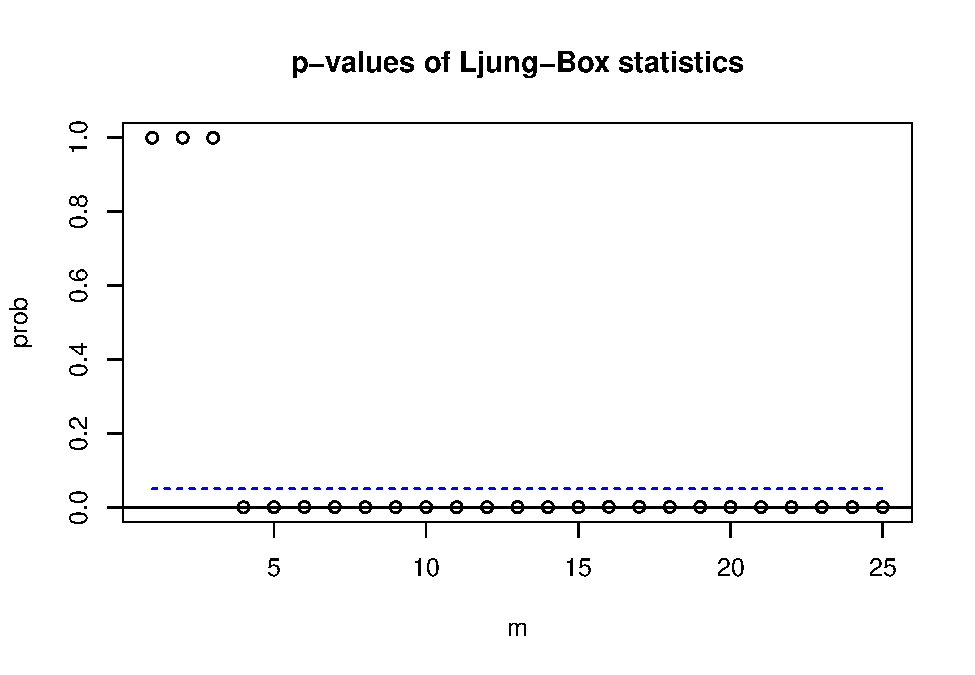
\includegraphics{solution_exercise_6_files/figure-latex/2_f-1.pdf}

\begin{Shaded}
\begin{Highlighting}[]
\KeywordTok{mq}\NormalTok{(var_}\FloatTok{3.}\NormalTok{ref.fit}\OperatorTok{$}\NormalTok{residuals, }\DataTypeTok{lag =} \DecValTok{25}\NormalTok{, }\DataTypeTok{adj =}\NormalTok{ ncoef.var_}\FloatTok{3.}\NormalTok{ref)}
\end{Highlighting}
\end{Shaded}

\begin{verbatim}
## Ljung-Box Statistics:  
##         m       Q(m)     df    p-value
##  [1,]   1.0      18.7    -5.0        1
##  [2,]   2.0      49.7    20.0        1
##  [3,]   3.0      77.4    45.0        0
##  [4,]   4.0     121.7    70.0        0
##  [5,]   5.0     145.3    95.0        0
##  [6,]   6.0     170.9   120.0        0
##  [7,]   7.0     196.3   145.0        0
##  [8,]   8.0     247.3   170.0        0
##  [9,]   9.0     284.0   195.0        0
## [10,]  10.0     320.4   220.0        0
## [11,]  11.0     352.0   245.0        0
## [12,]  12.0     391.7   270.0        0
## [13,]  13.0     415.2   295.0        0
## [14,]  14.0     446.0   320.0        0
## [15,]  15.0     458.6   345.0        0
## [16,]  16.0     481.5   370.0        0
## [17,]  17.0     517.0   395.0        0
## [18,]  18.0     544.1   420.0        0
## [19,]  19.0     573.6   445.0        0
## [20,]  20.0     614.0   470.0        0
## [21,]  21.0     636.7   495.0        0
## [22,]  22.0     669.2   520.0        0
## [23,]  23.0     694.9   545.0        0
## [24,]  24.0     726.9   570.0        0
## [25,]  25.0     756.4   595.0        0
\end{verbatim}

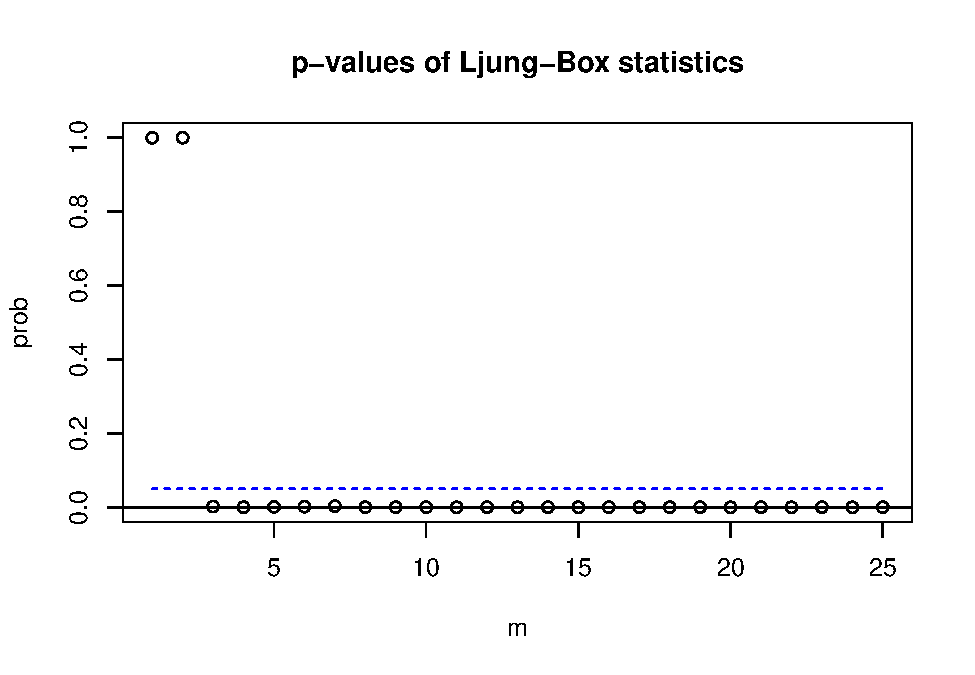
\includegraphics{solution_exercise_6_files/figure-latex/2_f-2.pdf}

\begin{Shaded}
\begin{Highlighting}[]
\CommentTok{# Well, both tests show depressing results. but by freeing up degrees of freedom, we can at least make a statement about m = 3 in the refined model}

\CommentTok{# some computation:}
\CommentTok{#ncoef.var4 / 5^2}
\CommentTok{#ncoef.var4.ref / 5^2}
\end{Highlighting}
\end{Shaded}

\end{document}
